
In this section, we discuss the performance of a cosmological
simulation code implemented using FDPS. We implemented TreePM (Tree
Particle-Mesh) method and measured the performance on XC30. Our TreePM
code is based on the code developed by K. Yoshikawa. The Particle-Mesh
part of the code was developed by
\citet{Ishiyama:2012:PAN:2388996.2389003} and this code is included in
the FDPS package as an external module.

We initially place particles uniformly in a cube and gave them zero
velocity. For the calculation of the tree force , we used a monopole
only kernel with cutoff. The cutoff length of the force is three times
larger than the width of the mesh. We set $\theta$ to 0.5. For the
calculation of the mesh force, the mass density is assigned to each of
the grid points, using the triangular shaped cloud scheme and the
density profile we used is the S2 profile \citep{hockney1988computer}.

Figures \ref{fig:cosmo_weak} and \ref{fig:cosmo_strong} show the weak
and strong scaling performance, respectively. For the weak-scaling
measurement, we fixed the number of particles per process to 5.73
million and measured the performance for the number of cores in the
range of 192 to 12000 on XC30. For the strong-scaling measurements, we
fixed the total number of particles to $2048^3$ and measured the
performance for the number of cores in the range of 1536 to 12000 on
XC30. We can see that the time for the calculation of the tree force
is dominant and both of the weak and strong scalings are good except
for the very large number of cores (12000) for the strong scaling
measurement. One reason is that the scalability of the calculation of
the mesh force is not very good. Another reason is that the time for
the domain decomposition grows linearly for large number of cores,
because we did not use parallelized domain decomposition here. The
efficiency is 7\% of the theoretical peak performance. It is rather
low compared to that for the disk galaxy simulations in
section \ref{sec:diskgalaxy}. The main reason is that we use a lookup
table for the force calculation. If we evaluate the force without the
lookup table, the nominal efficiency would be much better, but the
total time would be longer.

\begin{figure}
  \begin{center}
    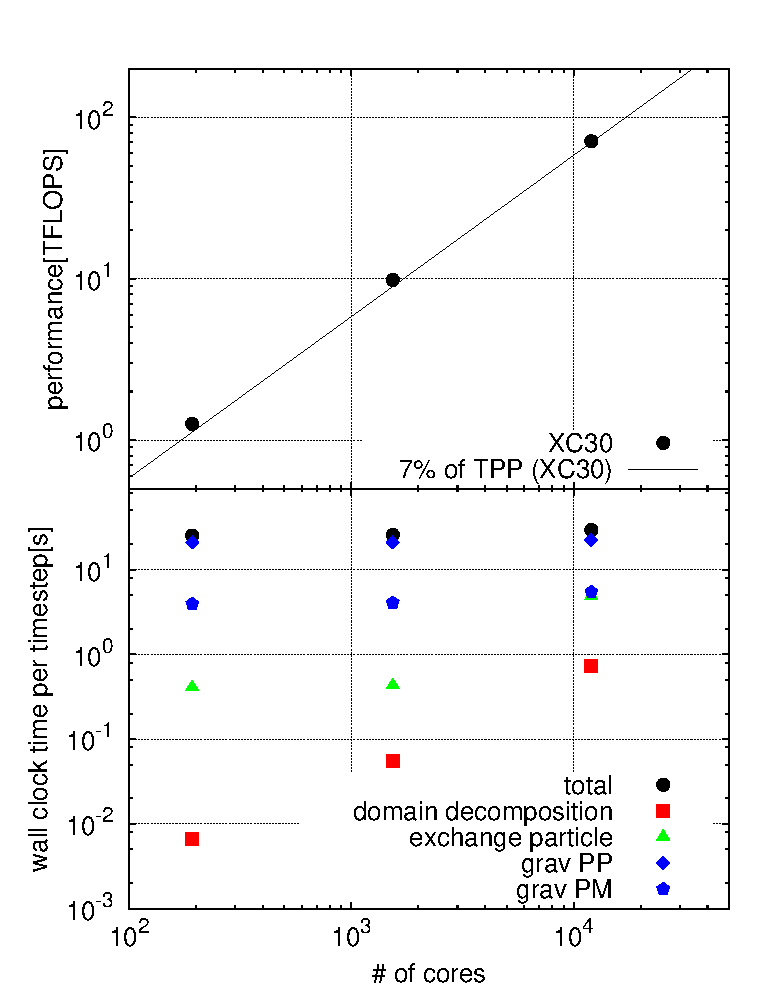
\includegraphics[width=8cm]{figure/cosmo_weak.eps}
  \end{center}
  \caption{

    Weak-scaling performance of the TreePM code. The speed of the
    floating-point operation (top) and wallclock time per one timestep
    (bottom) are plotted as functions of the number of cores. In the
    top panel, the solid line indicates 7\% of the theoretical peak
    performance of XC30. In the bottom panel, time spent for the
    Particle-Particle interaction calculation (diamond), the
    Particle-Mesh interaction (pentagon), the domain decomposition
    (square) and the exchange particles (triangle) are also shown.
    
  }
  \label{fig:cosmo_weak}
\end{figure}

\begin{figure}
  \begin{center}
    \includegraphics[width=8cm]{figure/cosmo_strong.eps}
  \end{center}
  \caption{

    The same as figure \ref{fig:cosmo_weak} but for the strong-scaling
    performance. In this case, the number of particles is $2048^3$.

  }
  \label{fig:cosmo_strong}
\end{figure}

